%%%%%%%%%%%%%%%%%%%%%%%%%%%%%%%%%%%%%%%%%
%
% (c) 2019 by Jennifer Laaser
%
% This work is licensed under the Creative Commons Attribution-NonCommercial-ShareAlike 4.0 International License. To view a copy of this license, visit http://creativecommons.org/licenses/by-nc-sa/4.0/ or send a letter to Creative Commons, PO Box 1866, Mountain View, CA 94042, USA.
%
% The current source for these materials is accessible on Github: https://github.com/jlaaser/pogil-polymers
%
%%%%%%%%%%%%%%%%%%%%%%%%%%%%%%%%%%%%%%%%%

\renewcommand{\figpath}{content/polymphys/mechanical-properties/SAOS/figs}
\renewcommand{\labelbase}{viscoelasticity}

\begin{activity}[extension]{Small-Amplitude Oscillatory Shear Rheology}

\begin{instructornotes}

	This activity introduces students to important concepts in small-amplitude oscillatory shear rheology.
	
	After completing this activity, students will be able to:
			\begin{enumerate}
				\item Explain what a small-amplitude oscillatory shear rheology experiment is
				\item Explain what the ``storage modulus'' and ``loss modulus'' of a material are
				\item Interpret data from a small-amplitude oscillatory shear rheology experiment in terms of the liquid- or solid-like properties of the material and the characteristic relaxation time
			\end{enumerate}
	
			
	\subsection*{Activity summary:}
	\begin{itemize}
		\item \textbf{Activity type:} Learning Cycle
		\item \textbf{Content goals:} Explaining SAOS experiments
		\item \textbf{Process goals:} %https://pogil.org/uploads/attachments/cj54b5yts006cklx4hh758htf-process-skills-official-pogil-list-2015-original.pdf
			\begin{itemize}
				\item Interpreting equations in terms of physical behavior
				\item Reading and interpreting graphs
			\end{itemize}
		\item \textbf{Duration:} approx. 30 min
		\item \textbf{Instructor preparation required:} 
			\begin{itemize}
				\item n/a
			\end{itemize}
		\item \textbf{Related textbook chapters:}
			\begin{itemize}
				\item \emph{Polymer Chemistry} (Hiemenz \& Lodge): Sections 11.2.4 and 11.8
			\end{itemize}
	\end{itemize}

\end{instructornotes}

	%\textbf{Focus question:} Put a central question for the students to consider through this exercise here.


\begin{model}[Small-Amplitude Oscillatory Shear Rheology]
\label{model:rheology}

	One of the most common experimental techniques used to characterize the viscoelasticity of polymeric materials is small-amplitude oscillatory shear rheology (SAOS).
	
	In a SAOS measurement, the sample is sandwiched between two surfaces that rotate back and forth at frequency $\omega$, resulting in a sinusoidally-varying strain:
	
	\vspace{0.1in}
	\begin{minipage}{0.15\textwidth}
	~
	\end{minipage}
	\begin{minipage}{0.35\textwidth}
		\centerline{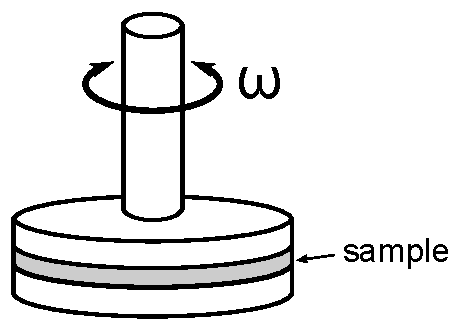
\includegraphics[width=0.9\textwidth]{\figpath/model1-parallelplates.pdf}}
	\end{minipage}
	\begin{minipage}{0.4\textwidth}
		\begin{equation*}
			\gamma(t) = \gamma_0 \sin(\omega t)
		\end{equation*}
	\end{minipage}
	\vspace{0.1in}
	
	The instrument (a rheometer) then measures the resulting stress as a function of time, $\sigma(t)$, and breaks it down into two components: one that is proportional to $\sin(\omega t)$ and one that is proportional to $\cos(\omega t)$. The response of the material can thus be expressed as follows:
	\begin{equation*}
		\frac{\sigma(t)}{\gamma_0} = G' \sin(\omega t) + G'' \cos(\omega t)
	\end{equation*}
	where we have normalized the stress, $\sigma(t)$, by the magnitude of the strain, $\gamma_0$.

\end{model}

%\vspace{0.25in}
\begin{ctqs}
		
		\question In this experiment, the strain is proportional to $\sin(\omega t)$.  
			\begin{enumerate}
				\item Which coefficient, $G'$ or $G''$, tells you how much of the response is directly proportional to the applied strain?
	
					\begin{solution}[1.1in]
						$G'$ is in the term that goes as $\sin(\omega t)$, so $G'$ is the coefficient that tells us how much of the response is directly proportional to the applied strain.
					\end{solution}
		
		\item Does this coefficient tell you about the elastic response of the material, or the viscous response of the material?
	
					\begin{solution}[1.1in]
						The elastic response is directly proportional to the applied strain, so this coefficient tells us about the elastic response.
					\end{solution}
					
			\end{enumerate}
		
		\question Since $\frac{d}{dt}\sin(\omega t) \sim \cos(\omega t)$, the strain \emph{rate} in this experiment is proportional to $\cos(\omega t)$.
		
			\begin{enumerate}
		
				\item Which coefficient, $G'$ or $G''$, tells you how much of the response is proportional to the strain rate?
	
					\begin{solution}[1.1in]
						The $G''$ term is proportional to $\cos(\omega t)$, so $G''$ tells us about the portion of the response that is proportional to strain rate.
					\end{solution}
		
				\item Does this coefficient tell you about the elastic response of the material, or the viscous response of the material?
	
					\begin{solution}[1.1in]
					
						The viscous response is proportional to the strain rate, so this coefficient tells us about the viscous repsonse.
					
					\end{solution}
					
			\end{enumerate}
		
		\question Remembering that elastic responses store energy, and viscous responses dissipate energy, explain why we call $G'$ the ``storage modulus'' and $G''$ the ``loss modulus'' of the material.
	
					\begin{solution}[2in]
					
						$G'$ gives information about the elastic response, which stores energy, so $G'$ is called the storage modulus.
						
						$G''$ gives information about the viscous response, which dissipates energy, so $G''$ is called the loss modulus.
					\end{solution}
			
\end{ctqs}

\clearpage
\begin{model}[Dynamic Moduli of the Maxwell Model]
\label{\labelbase:mdl:dynamicmoduli}
	As shown in Exercise \ref{\labelbase:exc:Boltzmann}, the storage and loss moduli for the Maxwell Model are given by:
	\begin{align*}
		G' = G_0 \frac{\omega^2 \tau^2}{\omega^2 \tau^2 + 1} && \text{and} && G'' = G_0 \frac{\omega \tau}{\omega^2 \tau^2 + 1}
	\end{align*}
	
	A plot of these moduli as a function of frequency is given below:
			
		\vspace{0.1in}	
		\centerline{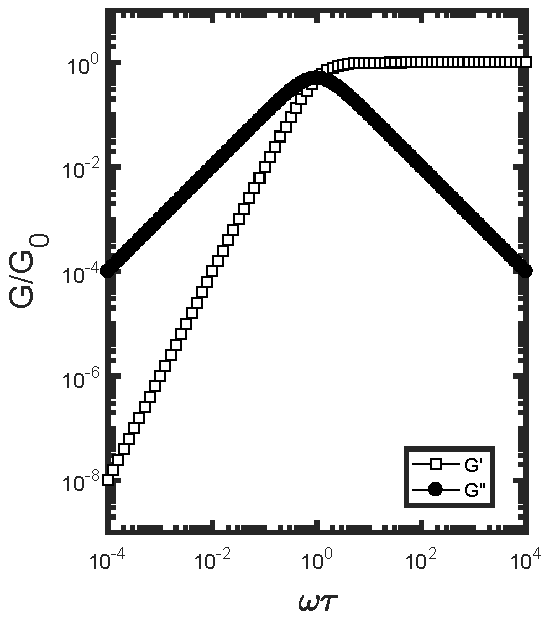
\includegraphics[width=0.4\textwidth]{\figpath/model2-maxwellplot}}
	
	Note that both axes of this graph are plotted on a log scale; the x axis has been scaled by the characteristic relaxation time, $\tau$, and the y axis has been scaled by the modulus, $G_0$.
	
\end{model}

\begin{ctqs}
	
	\question First, consider the low-frequency portion of the response:
	
		\begin{enumerate}
		
			\item  At low frequencies, which is larger, the storage modulus or the loss modulus?
	
					\begin{solution}[1in]
					
						According to the plot, the loss modulus is larger at low frequencies.
					
					\end{solution}
					
			\item Do low frequency measurements correspond to fast (short) timescales, or long (slow) timescales?
			
				\begin{solution}[1in]
				
					Low-frequency measurements correspond to long timescales, because it takes a long time for a single oscillation to take place.
				
				\end{solution}
					
			\item Are your answers to the preceding two questions consistent with your understanding of the relationships between the characteristic relaxation time, the timescale of observation, and the type of properties you should observe?  Explain your reasoning in 1-2 complete sentences.
			
				\begin{solution}[2in]
				
					Yes. As we learned in the last activity, the Maxwell model should give liquid-like behavior on long timescales, which correspond to low frequencies.  Thus it makes sense that the loss modulus (corresponding to liquid-like behavior) should dominate at low frequencies.
				
				\end{solution}
	
		\end{enumerate}
	
	\question Now, consider the high-frequency portion of the response:
	
		\begin{enumerate}
		
			\item At high frequencies, which is larger, the storage modulus or the loss modulus?
	
					\begin{solution}[1in]
					
						According to the plot, the storage modulus is larger at high frequencies.
					
					\end{solution}
					
			\item Do high frequency measurements correspond to fast (short) timescales, or long (slow) timescales?
			
				\begin{solution}[1in]
				
					High-frequency measurements correspond to fast timescales, because it takes very little time time for a single oscillation to take place.
				
				\end{solution}
					
			\item Are your answers to the preceding two questions consistent with your understanding of the relationships between the characteristic relaxation time, the timescale of observation, and the type of properties you should observe?  Explain your reasoning in 1-2 complete sentences.
			
				\begin{solution}[2in]
				
					Yes. As we learned in the last activity, the Maxwell model should give solid-like behavior on short timescales, which correspond to high frequencies.  Thus it makes sense that the storage modulus (corresponding to solid-like behavior) should dominate at high frequencies.
				
				\end{solution}
	\end{enumerate}

	\question At what frequency is the storage modulus exactly equal to the loss modulus?  Give your answer in terms of the characteristic relaxation time, $\tau$.
	
		\emph{Note: you can answer this question using either the graph or the equations, but you will probably find it easier to work from the equations.}
	
					\begin{solution}[1.75in]
					
						Setting the equations for $G'$ and $G''$ equal to each other, we have
						\begin{align*}
							G' &= G''\\
							G_0 \frac{\omega^2 \tau^2}{\omega^2 \tau^2 + 1} &= G_0 \frac{\omega \tau}{\omega^2 \tau^2 + 1}\\
							\omega^2 \tau^2 &= \omega \tau\\
							\omega\tau &= 1\\
							\omega &= \frac{1}{\tau}
						\end{align*}
					\end{solution}
	
	\question The frequency identified in the previous question is called the ``crossover frequency'', because it is where the plots for $G'$ and $G''$ cross each other.
	
		\begin{enumerate}
			\item Rearrange your answer to the previous question to find an expression for the characteristic relaxation time in terms of the crossover frequency.
	
					\begin{solution}[1in]
					
						\begin{align*}
							\tau = \frac{1}{\omega_c}
						\end{align*}
					\end{solution}
					
			\item Propose a method you could use to identify the characteristic relaxation time of a material from an SAOS measurement.  Describe your proposed method in 2-3 complete sentences.
			
				\begin{solution}[2.5in]
					First, look at the plot of the dynamic moduli and find the frequency at which the storage and loss moduli are equal.					
					Then, calculate the inverse of this frequency.  The result will be the characteristic relaxation time of the material.
					
					\emph{Note for instructors: this analysis only strictly holds for the Maxwell model.  For real polymeric materials that have multiple relaxation timescales, this procedure typically \emph{underestimates} the longest relaxation time of the sample.}
				\end{solution}
			
		\end{enumerate}
	
\end{ctqs}
	

\clearpage
\begin{exercises}

\exercise Consider the polymer characterized in the following plot:
				
		\centerline{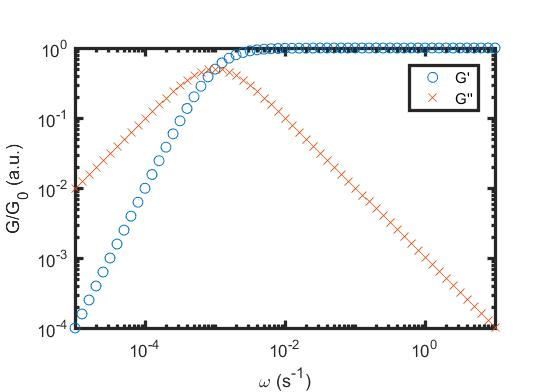
\includegraphics[width=0.6\textwidth]{\figpath/exercise-maxwellexample.jpg}}
		
		\begin{enumerate}
		
			\item Find the characteristic relaxation time of this polymer.
	
					\begin{solution}\instructordisplay{
					
						The storage and loss moduli are equal when $\omega=10^{-3}\text{ s}^{-1}$.  Thus the characteristic relaxation time is
						
						\begin{equation*}
							\tau = \frac{1}{\omega_c} = \frac{1}{10^{-3}\text{ s}^{-1}} = 1000\text{ s} \approx 17\text{ min}
						\end{equation*}
					}\end{solution}
	
			\item If you were to pick up a sample of this polymer, would you expect it to feel more like a liquid or more like a solid?  Briefly justify your answer.
	
			\emph{Hint: think about how the timescale on which you are observing/interacting with the polymer compares to the relaxation time!}
	
					\begin{solution}\instructordisplay{
					
						This polymer would probably feel more like a solid.  When we pick a material up, we are typically observing it on timescales on the order of a second.  This timescale is much shorter than the characteristic relaxation time of the material, so we will observe primarily solid-like properties.
					
					}\end{solution}
					
		\end{enumerate}

		\exercise \label{\labelbase:exc:Boltzmann} In the previous activity we considered step-strain experiments, while in this activity, we considered oscillatory strain experiments.  As it turns out, we can \emph{use} the step-strain result to \emph{derive} the oscillatory strain result via the \emph{Boltzmann superposition principle}.
		
			The Boltzmann superposition principle says that we can effectively break down the time-dependent strain into a series of step strains, each of which has their own stress response:
				
		\centerline{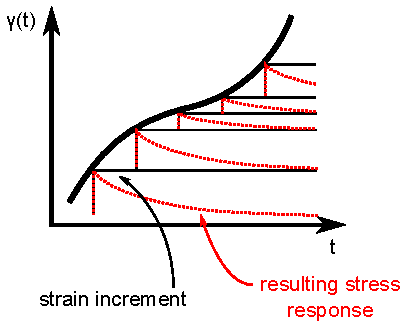
\includegraphics[width=0.4\textwidth]{\figpath/exercise-boltzmann.pdf}}
			
			The total stress response of the material is then the sum of each of these individual responses.
			
			Mathematically, we find that for a material whose response to a step strain of size $\gamma_0$ is given by $\sigma(t) = G(t)\gamma_0$, the response to an arbitrary strain $\gamma(t)$ is given by
			\begin{equation*}
				\sigma(t) = \int_0^{\infty} G(t') \dot\gamma(t-t') dt'
			\end{equation*}
		
			\begin{enumerate}
			
				\item Use this equation to find an expression for $\sigma(t)$ for a material with an arbitrary stress relaxation modulus $G(t)$ undergoing oscillatory strain of the form $\gamma(t) = \gamma_0 \sin(\omega t)$.
				
					\emph{Hint: to make the next step easier, you will want to rewrite the $\cos$ term in the integral using the angle addition formula $\cos(a+b) = \cos(a)\cos(b) + \sin(a)\sin(b)$.}
				
					\begin{solution}\instructordisplay{
					
						First, we need to calculate $\dot\gamma(t)$:
						\begin{align*}
							\dot\gamma(t) &= \frac{d}{dt}\gamma_0\sin(\omega t) \\
							 &= \gamma_0 \omega \cos(\omega t)
						\end{align*}
						
						Next, we need to plug this into the expression for $\sigma(t)$ given in the problem:
						\begin{align*}
							\sigma(t) &= \int_0^{\infty} G(t') \dot\gamma(t-t') dt'\\
								&= \int_0^{\infty} G(t') \gamma_0 \omega\cos(\omega(t-t')) dt'\\
								&= \gamma_0 \omega \int_0^{\infty} G(t') \cos(\omega(t-t')) dt'
						\end{align*}
						
						Finally, expanding the cosine term, we have:
						\begin{align*}
							\sigma(t) &= \gamma_0 \omega\int_0^{\infty} G(t') \cos(\omega t-\omega t') dt'\\
								&= \gamma_0 \omega \int_0^{\infty} G(t') \left(\cos(\omega t)\cos(\omega t') + \sin(\omega t)\sin(\omega t')\right) dt'
						\end{align*}
						
					}\end{solution}
				
				\item Use your result to find expressions for the storage and loss moduli, $G'(\omega)$ and $G''(\omega)$, of the material.
				
					\begin{solution}\instructordisplay{
					
						Rearranging our result from the previous problem, we can write $\sigma(t)$ as the sum of a term that goes as $\cos(\omega t)$ and  a term that goes as $\sin(\omega t)$ as follows:
						\begin{align*}
							\sigma(t) &= \gamma_0 \omega \int_0^{\infty} G(t') \cos(\omega t)\cos(\omega t')dt' + \gamma_0 \omega \int_0^{\infty} G(t') \sin(\omega t)\sin(\omega t') dt'\\
								&= \left[\gamma_0 \omega \int_0^{\infty} G(t') \cos(\omega t')dt'\right]\cos(\omega t) + \left[\gamma_0 \omega \int_0^{\infty} G(t') \sin(\omega t') dt'\right]\sin(\omega t)
						\end{align*}
						Note that the second step of this manipulation requires students to recognize that the $\sin(\omega t)$ and $\cos(\omega t)$ terms can be pulled out of the integral since they do not contain the integration variable, $t'$; some students may get stuck on this point.
						
						Recall from the beginning of the activity that
						\begin{equation*}
							\frac{\sigma(t)}{\gamma_0} = G' \sin(\omega t) + G'' \cos(\omega t)
						\end{equation*}
						For our expression for $\sigma(t)$, we find that
						\begin{equation*}
							\frac{\sigma(t)}{\gamma_0} = \left[ \omega \int_0^{\infty} G(t') \cos(\omega t')dt'\right]\cos(\omega t) + \left[ \omega \int_0^{\infty} G(t') \sin(\omega t') dt'\right]\sin(\omega t)
						\end{equation*}
						
						Setting the coefficients of the sine terms equal to each other, we find that
						\begin{align*}
							%G' &= \left[\omega \int_0^{\infty} G(t') \sin(\omega t') dt'\right] \\
							G'(\omega) &= \omega \int_0^{\infty} G(t') \sin(\omega t') dt'
						\end{align*}
						and similarly, setting the coefficients of the cosine terms equal to each other, we find that
						\begin{align*}
							%G'' &= \left[\omega \int_0^{\infty} G(t') \cos(\omega t')dt'\right] \\
							G''(\omega) &= \omega \int_0^{\infty} G(t') \cos(\omega t')dt'
						\end{align*}
						
						Students who have seen Fourier transforms in previous classes may recognize that the dynamic moduli are simply the sine and cosine transforms of the stress relaxation modulus, $G(t)$.
						
					}\end{solution}
			
				\item What is $G(t)$ for the Maxwell model? \emph{(Recall that for the Maxwell model, the initial stress, $\sigma_0$, is equal to $G_0\gamma_0$.)}
				
					\begin{solution}\instructordisplay{
						For the Maxwell model, the step-stress response is
						\begin{equation*}
							\sigma(t) = \sigma_0 e^{-t/\tau}
						\end{equation*}
						Setting this equal to $G(t)\gamma_0$, we find
						\begin{align*}
							G(t) &= \frac{\sigma_0}{\gamma_0} e^{-t/\tau}\\
								&= G_0 e^{-t/\tau}
						\end{align*}
					}\end{solution}
			
				\item Use your answers to the preceding two questions to calculate $G'(\omega)$ and $G''(\omega)$ for the Maxwell model, and verify that your answer are consistent with the results given in Model \ref{\labelbase:mdl:dynamicmoduli}.
				
					\begin{solution}\instructordisplay{
					
						For the storage modulus, we find that
						\begin{align*}
							G'(\omega) &= \omega \int_0^{\infty} G_0 e^{-t/\tau} \sin(\omega t') dt'\\ 
								&= G_0 \omega \int_0^{\infty} e^{-t/\tau} \sin(\omega t') dt'
						\end{align*}
						From a standard table of integrals (or Wolfram Alpha), we obtain
						\begin{align*}
							\int_0^{\infty} e^{-ax}\sin(b x)dx = \frac{b}{a^2 + b^2}
						\end{align*}
						Thus, with $a = \frac{1}{\tau}$ and $b = \omega$,
						\begin{align*}
							G'(\omega) &= G_0 \omega \frac{\omega}{\left(\frac{1}{\tau}\right)^2 + \omega^2} \\
								&= G_0 \frac{\omega^2\tau^2}{1+\omega^2\tau^2}
						\end{align*}
						which is exactly the result given in Model \ref{\labelbase:mdl:dynamicmoduli}.
						
						}\end{solution}		%  necessary to fix page break issues
						\begin{solution}\instructordisplay{
						
						Similarly, for the loss modulus, we find that
						\begin{align*}
							G''(\omega) &= \omega \int_0^{\infty} G_0 e^{-t/\tau} \cos(\omega t') dt'\\ 
								&= G_0 \omega \int_0^{\infty} e^{-t/\tau} \cos(\omega t') dt'
						\end{align*}
						From a standard table of integrals (or Wolfram Alpha), we obtain
						\begin{align*}
							\int_0^{\infty} e^{-ax}\cos(b x)dx = \frac{a}{a^2 + b^2}
						\end{align*}
						Thus, with $a = \frac{1}{\tau}$ and $b = \omega$,
						\begin{align*}
							G'(\omega) &= G_0 \omega \frac{\frac{1}{\tau}}{\left(\frac{1}{\tau}\right)^2 + \omega^2} \\
								&= G_0 \frac{\omega\tau}{1+\omega^2\tau^2}
						\end{align*}
						which is, again, exactly the result given in Model \ref{\labelbase:mdl:dynamicmoduli}.
						
						
					}\end{solution}
				
			\end{enumerate}

		
		
\end{exercises}
	
\end{activity}